\section{Spark::Sp\-Stream\-Geometry Class Reference}
\label{classSpark_1_1SpStreamGeometry}\index{Spark::SpStreamGeometry@{Spark::SpStreamGeometry}}
{\tt \#include $<$Sp\-Stream\-Geometry.h$>$}

Inheritance diagram for Spark::Sp\-Stream\-Geometry:\begin{figure}[H]
\begin{center}
\leavevmode
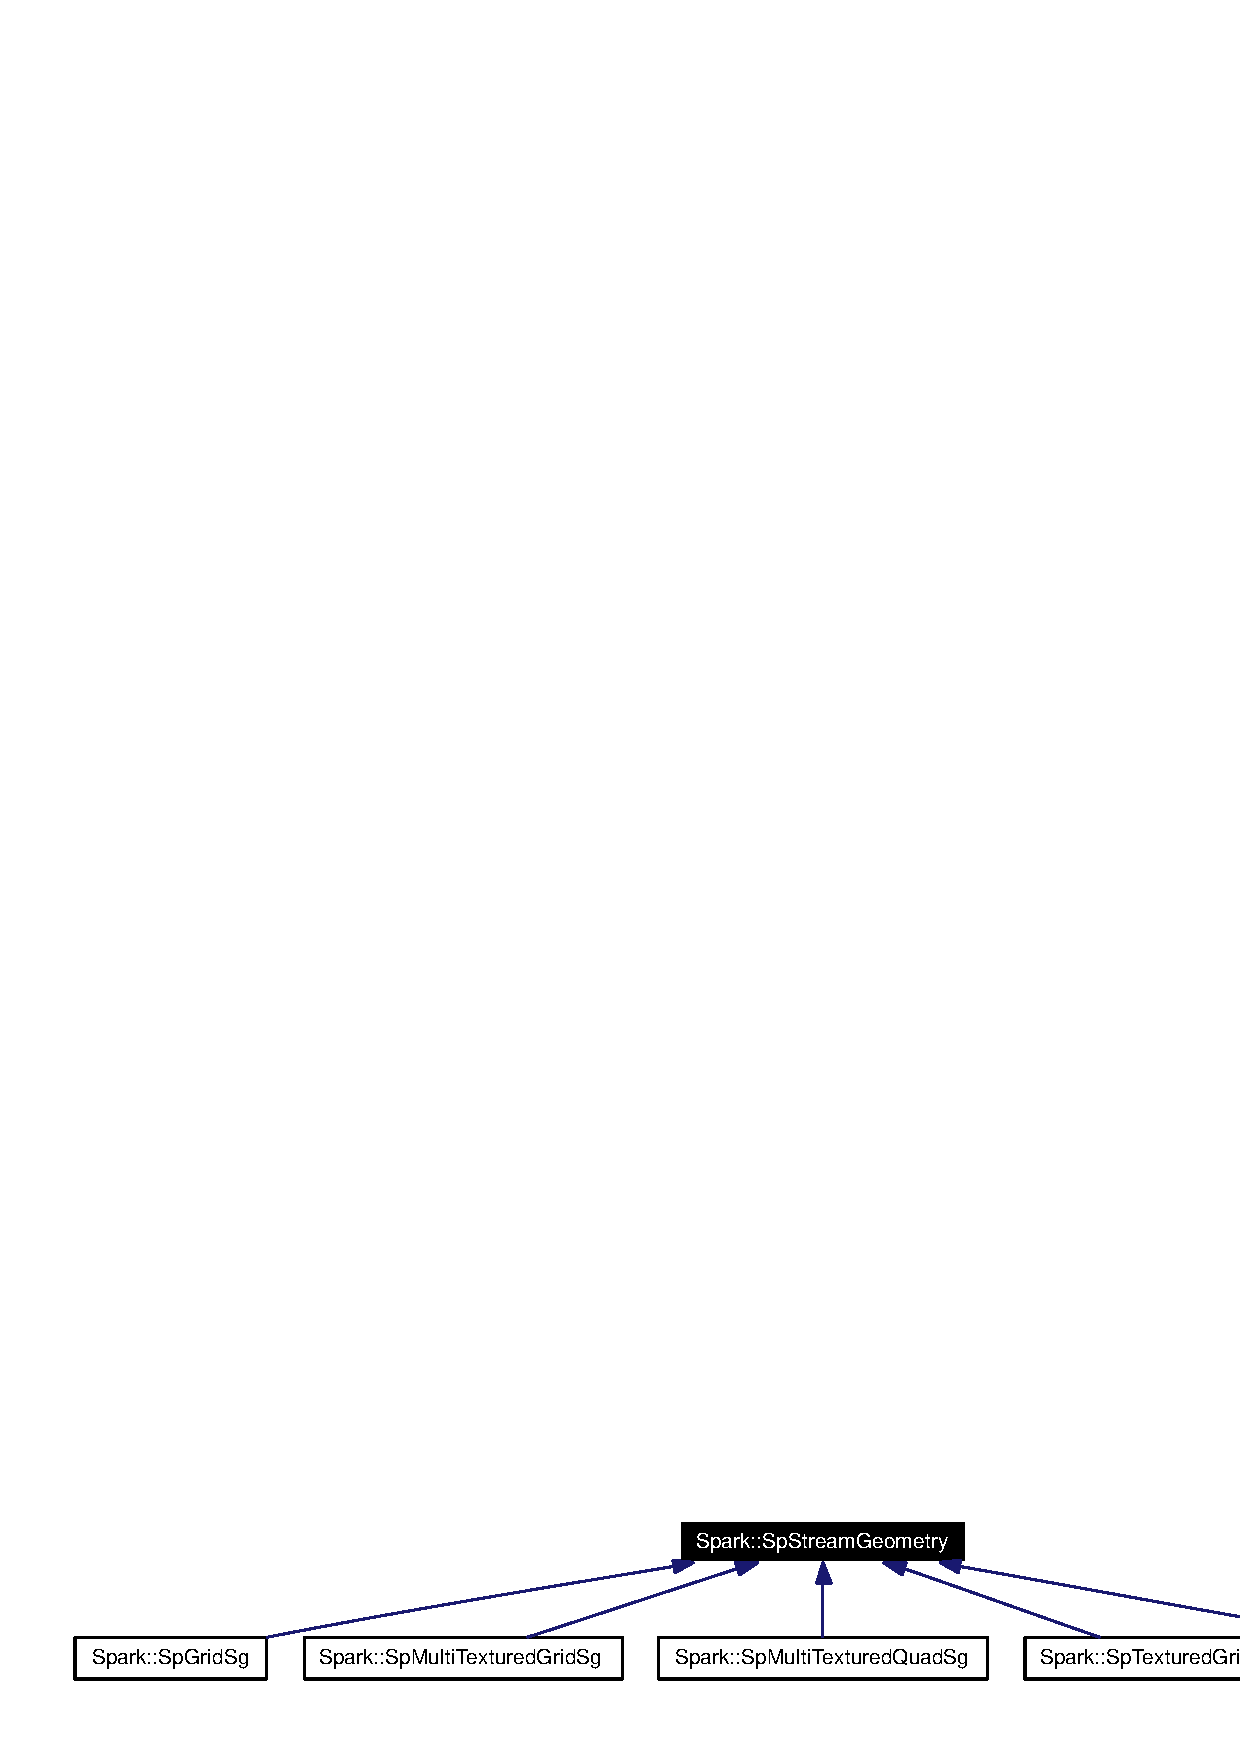
\includegraphics[width=388pt]{classSpark_1_1SpStreamGeometry__inherit__graph}
\end{center}
\end{figure}


\subsection{Detailed Description}
Abstract base class for generating a data stream by rendering geometry. 

Definition at line 30 of file Sp\-Stream\-Geometry.h.\subsection*{Public Member Functions}
\begin{CompactItemize}
\item 
virtual void {\bf render} ()=0
\begin{CompactList}\small\item\em Renders geometry to generate a data stream. \item\end{CompactList}\end{CompactItemize}


\subsection{Member Function Documentation}
\index{Spark::SpStreamGeometry@{Spark::Sp\-Stream\-Geometry}!render@{render}}
\index{render@{render}!Spark::SpStreamGeometry@{Spark::Sp\-Stream\-Geometry}}
\subsubsection{\setlength{\rightskip}{0pt plus 5cm}virtual void Spark::Sp\-Stream\-Geometry::render ()\hspace{0.3cm}{\tt  [pure virtual]}}\label{classSpark_1_1SpStreamGeometry_a0}


Renders geometry to generate a data stream. 



Implemented in {\bf Spark::Sp\-Grid\-Sg} {\rm (p.\,\pageref{classSpark_1_1SpGridSg_a2})}, {\bf Spark::Sp\-Multi\-Textured\-Grid\-Sg} {\rm (p.\,\pageref{classSpark_1_1SpMultiTexturedGridSg_a2})}, {\bf Spark::Sp\-Multi\-Textured\-Quad\-Sg} {\rm (p.\,\pageref{classSpark_1_1SpMultiTexturedQuadSg_a2})}, {\bf Spark::Sp\-Textured\-Grid\-Sg} {\rm (p.\,\pageref{classSpark_1_1SpTexturedGridSg_a2})}, and {\bf Spark::Sp\-Textured\-Quad\-Sg} {\rm (p.\,\pageref{classSpark_1_1SpTexturedQuadSg_a2})}.



The documentation for this class was generated from the following file:\begin{CompactItemize}
\item 
{\bf Sp\-Stream\-Geometry.h}\end{CompactItemize}
